\chapter{Communication Protocols}
Before going deeply into details of the project, wired and wireless communication protocols have to be discussed since the project is considered as communication system, so this chapter shows how communication protocols are used in the project, and why was each one chosen. Wired communications that will be discussed are UART, I2C, and SPI, and these protocols are important to communicate between the prototype of the project and the sensors, CAN protocols is also discussed since it plays an important role in the modern cars. This chapter will also explain wireless communication protocols such as Wi-Fi and Bluetooth.

\section{Wired Communication Protocols}
Wired communication is an efficient method to communicate between nearby devices, thus the usage of wired communication appears in V2V vehicle unit since it helps to communicate between sensors/modules and the processor.
In this section UART, I2C, SPI, and CAN are discussed through the following points:
\begin{enumerate}
    \item Background
    \item Why it is being used?
    \item Interfacing
\end{enumerate}
\subsection{UART}
There was a time when keyboards, mouse, and printers all had large cords and clumsy connectors. These must be inserted into the computer with a screwdriver. To interact with computers, these devices used UART. Although USB has replaced these clumsy wires, UARTs are still used in Do It Yourself (DIY) electronics like the Raspberry Pi, Arduino, and other ubiquitous microcontrollers. It can be used to link Bluetooth and GPS modules together. \newline
Other communication protocols, such as SPI and I2C, use a different transfer methodology than UART. In a microcontroller, it is a physical circuit. It can also work on its own as an integrated circuit. The fact that UART only uses two wires to carry data is a huge advantage. \clearpage
\subsubsection{1. Background of UART}
\begin{wrapfigure}{r}{5cm}
    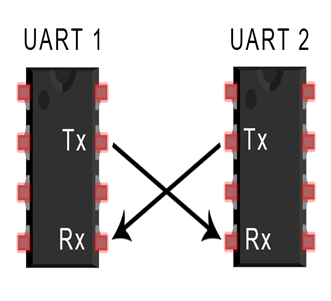
\includegraphics[width=0.25\textwidth]{figure/3_1.png}
    \caption{Connection between two devices using UART}
    \label{fig:connection-two-devices}
\end{wrapfigure}
Two UARTs communicate directly with each other in UART communication. The transmitting UART translates parallel data from a controlling device, such as a CPU, into serial data and sends it to the receiving UART, which then converts the serial data back into parallel data for the receiving device. To send data between two UARTs, only two wires are required. Data transfers from the transmitting UART's Tx pin to the receiving UART's Rx pin as shown in figure \ref{fig:connection-two-devices}.
\subsubsection{Transmitting and receiving serial data}
The transmitting UART takes bytes of data and transmits the bits in a sequential form. The second transmitter which is the receiver reassembles the bits into a complete byte. Serial transmission of data through a single wire is more cost-effective than parallel transmission through multiple wires. \newline
Simplex, full-duplex, or half-duplex communication between two UART devices is possible. Simplex communication is one-way communication in which the signal travels from one UART to the next. The receiving UART does not have the ability to send back signals. When both devices can transmit and receive data at the same time, it is called full-duplex. When devices communicate and receive data in half-duplex mode, they take turns transmitting and receiving data. \newline
\subsubsection{Steps of the UART transmission}
\begin{itemize}
    \item The transmitting UART receives data in parallel from the data bus.
    \item The transmitting UART adds the start bit, parity bit, and the stop bit(s) to the data frame.
    \item The entire packet is sent serially from the transmitting UART to the receiving UART. 
    \item The receiving UART samples the data line at the pre-configured baud rate.
    \item The receiving UART discards the start bit, parity bit, and stop bit from the data frame:
    \item The receiving UART converts the serial data back into parallel and transfers it to the data bus on the receiving end.
\end{itemize}
\clearpage
\subsubsection{Structure of a UART Protocol}
UART Packet as shown in figure \ref{fig:UART-packet} consists of 4 parts; start bit, data bit/s, parity bit/s, and stop bit/s.
\begin{figure}[h]
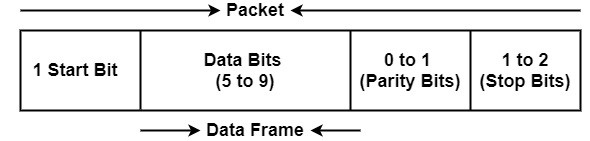
\includegraphics[width=\textwidth]{figure/3_2.jpg}
\caption{UART Packet}
\label{fig:UART-packet}
\centering
\end{figure}

\begin{itemize}
    \item \textbf{Start Bit: } Start-bit is also referred to as a synchronization bit that is located before the actual data. Usually, an inactive data transmission line is reserved at a high-voltage level. To start the data transmission, the UART transmission burden the data line from a high voltage level (1) to a low voltage level (0).
    \item \textbf{Stop Bit: } The Stop Bit is located at the ending of the data packet. Generally, this bit is 2-bits lengthy but commonly on bit only used. It can stop the broadcast, the UART maintains the data-line on high voltage.
    \item \textbf{Parity Bit: } The symmetry or oddness of a number is described by parity. The receiving UART uses the parity bit to determine if any data has changed during transmission. Electromagnetic radiation, mismatched baud rates, and long-distance data transfers can all alter bits. After reading the data frame, the receiving UART counts the number of bits with a value of 1 and determines whether the total is even or odd. The 1 bit in the data frame should amount to an even number if the parity bit is a 0 (even parity). The 1 bit in the data frame should amount to an odd number if the parity bit is a 1 (odd parity). The UART understands that the transmission was error-free when the parity bit matches the data. The UART knows that bits in the data frame have changed if the parity bit is a 0 and the total is odd; or if the parity bit is a 1 and the total is even. Briefly Parity bit allows the receiver to provide whether the collected record is right or not. It is a low-level fault checking system & parity bit is accessible in two ranges including Even Parity and Odd Parity.
    \item \textbf{Data Bits or Data Frame: } The data frame contains the actual data being transferred. It can be 5 bits up to 8 bits long if a parity bit is used. If no parity bit is used, the data frame can be 9 bits long. In most cases, the data is sent with the least significant bit first.
\end{itemize}

\subsubsection{2. Why UART is being used?}
\begin{enumerate}
    \item Low hardware complexity.
    \item Software addressing is not necessary because this connection is one to one between the two devices.
    \item It is often utilized in devices using 9 pin connectors due to its simplicity
\end{enumerate}

\subsubsection{3. Interfacing with UART}
In this project, UART protocol is used to interface between:
\begin{enumerate}
    \item Raspberry and STM: they transmit/receive data between them using UART protocol, Raspberry receives the output vehicle data from the STM to send them to the server, and it transmits the data came from Server to STM to pe processed and analyzed as will be shown in chapter 5.
    \item Bluetooth module and STM: In order to use GPS data, Bluetooth module is used since it connects to a mobile phone by Bluetooth using android application called “GPS share Data”, and in other side, it connects with STM and communicate with it by UART.
\end{enumerate}

Figure \ref{fig:interface-stm-rasp-bluetooth} shows how the connection is between STM and both the Bluetooth module and Raspberry; STM connects with Raspberry by UART2 whose pins are PA2 (Tx) and PA3 (Rx), PA2 is connected to Rx in Raspberry, and PA3 is connected to Tx, for Bluetooth module UART3 is used whose pins are PB10 (Tx) and PB11 (Rx), PB10 is connected to RX in the module, and PB11 is connected to Tx.

\begin{figure}[h]
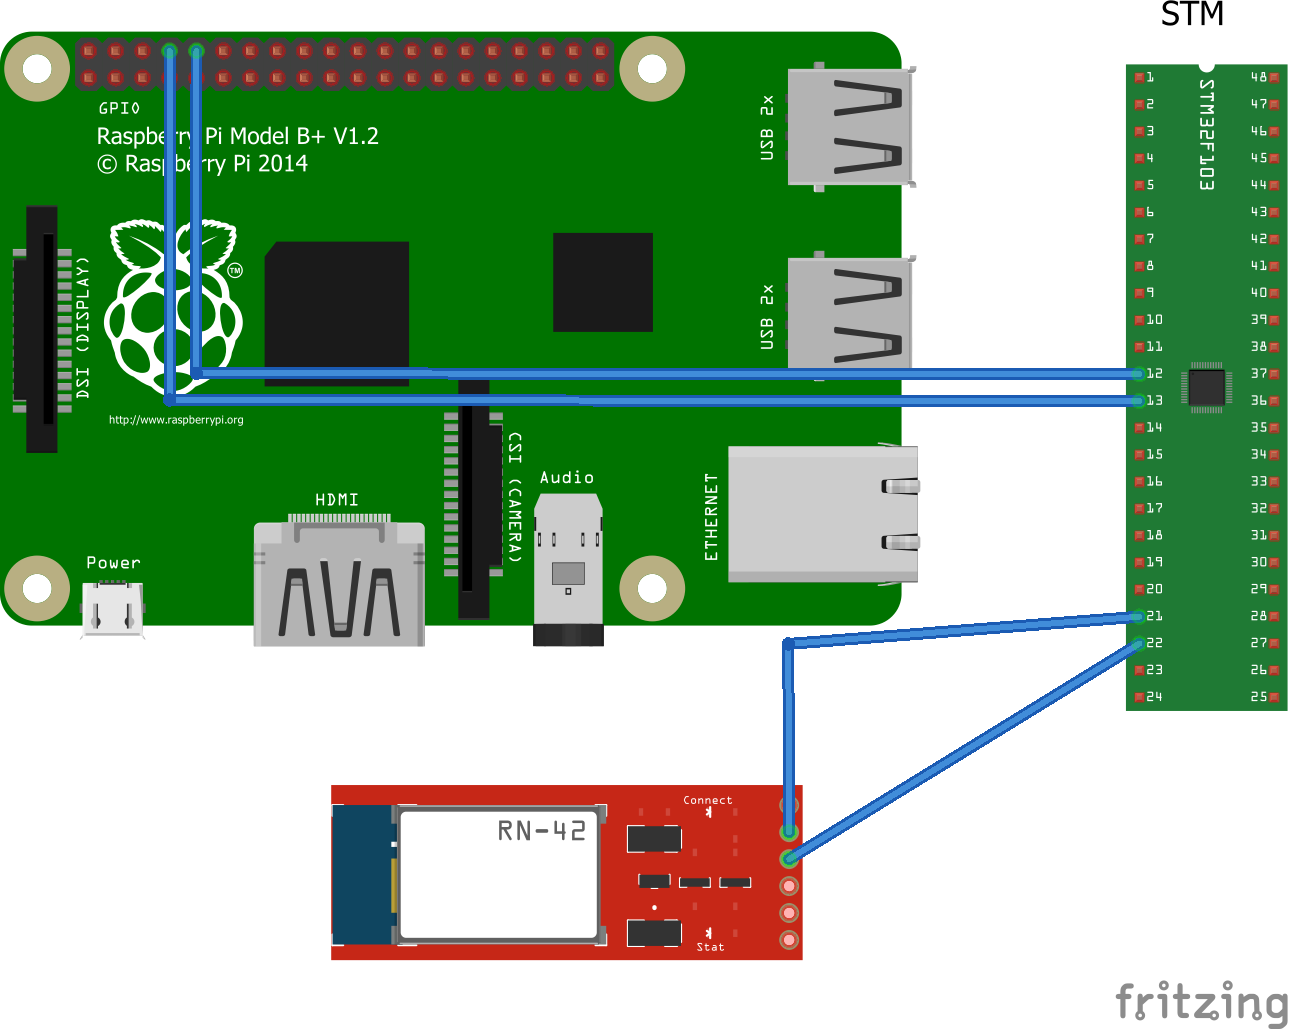
\includegraphics[width=\textwidth]{figure/3_3.png}
\caption{Intefcaing between STM and both Raspberry Pi and Bluetooth module}
\label{fig:interface-stm-rasp-bluetooth}
\centering
\end{figure}

\subsection{I2C}
Inter-Integrated Circuit is the acronym for it. It is a serial communication bus interface connection protocol used by devices. Philips Semiconductor created it at first in 1982. It has been a popular protocol recently for short-distance communication. It also goes by the name Two Wired Interface (TWI).

\subsubsection{1. Background of I2C}
Like UART communication, I2C only uses two wires to transmit data between devices as shown in figure \ref{fig:connectiong-i2c}. The main device is called Master (which is responsible for genrating a clock signal), and the second device is called Slave. Each device has two pins; SDA and SCL, SDA refers to select data, SCL refers to select clock line. The bus between SDAs pins is to transfer the data between two devices, and the bus between SCLs pin is to provide the clock for the slave device. 

\begin{figure}[h]
   \centering
    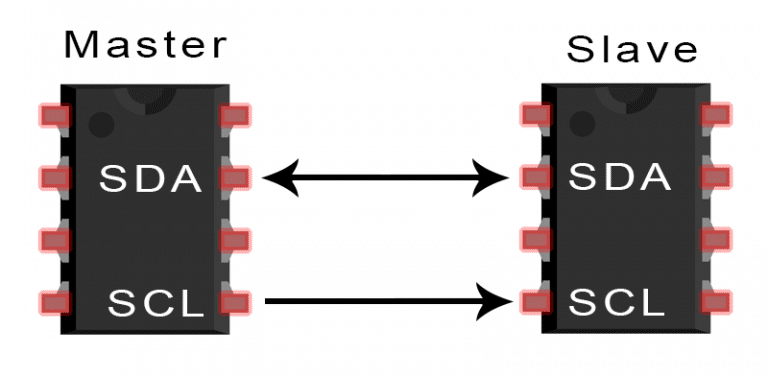
\includegraphics[width=0.5\textwidth]{figure/3_4.png}
    \caption{Connection between two devices using I2C}
    \label{fig:connectiong-i2c}
\end{figure}

\subsubsection{I2C Modes & Bus Speeds}
Originally, the I2C-bus was limited to 100 kbit/s operations. Over time there have been several additions to the specification so that there are now five operating speed categories. Standard-mode, Fast-mode (Fm), Fast-mode Plus (Fm+), and High-speed mode (Hs-mode) devices are downward compatible. This means any device may be operated at a lower bus speed. Ultra Fast-mode devices are not compatible with previous versions since the bus is unidirectional.
\begin{enumerate}
    \item Bidirectional bus:
    \begin{itemize}
        \item Standard-Mode (Sm), with a bit rate up to 100 kbit/s 
        \item Fast-Mode (Fm), with a bit rate up to 400 kbit/s
        \item Fast-Mode Plus (Fm+), with a bit rate up to 1 Mbit/s 
        \item High-speed Mode (Hs-mode), with a bit rate up to 3.4 Mbit/s. 
    \end{itemize}
    \item Unidirectional bus: 
    \begin{itemize}
        \item Ultra Fast-Mode (UFm), with a bit rate up to 5 Mbit/s 
    \end{itemize}
\end{enumerate}
Both SDA and SCL are bidirectional lines, connected to a positive supply voltage via a current source or pull-up resistor. When the bus is free, both lines are HIGH. The output stages of devices connected to the bus must have an open-drain or open-collector to perform the wired-AND function. \newline

\subsubsection{I2C working abstract}
With I2C, data is transferred in messages, Messages are broken up into frames of data. \newline
I2C message as shown in figure \ref{fig:i2c-message} has an address frame that contains the binary address of the slave, and one or more data frames that contain the data being transmitted. The message also includes start and stop conditions, read/write bits, and ACK/NACK bits between each data frame. \newline
\begin{figure}[h]
   \centering
    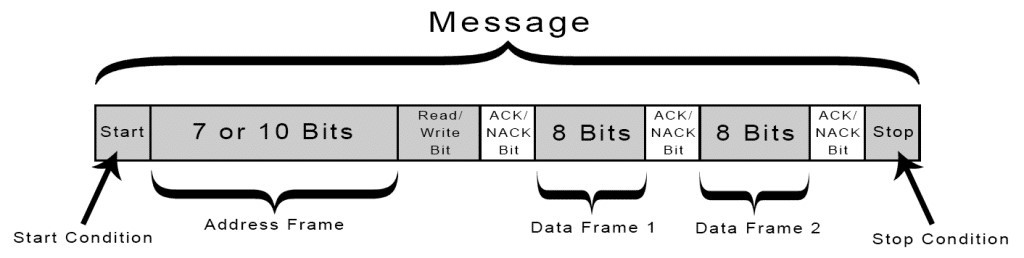
\includegraphics[width=.5\textwidth]{figure/3_5.jpg}
    \caption{I2C Message}
    \label{fig:i2c-message}
\end{figure}

\begin{itemize}
    \item \textbf{Start Condition: } The SDA line switches from a high voltage level to a low voltage level before the SCL line switches from high to low.
    \item \textbf{Stop Condition: } The SDA line switches from a low voltage level to a high voltage level after the SCL line switches from low to high. 
    \item \textbf{Address Frame: }  A 7- or 10-bit sequence unique to each slave that identifies the slave when the master wants to talk to it. 
    \item \textbf{Read/Write Bit: }  A single bit specifying whether the master is sending data to the slave (low voltage level) or requesting data from it (high voltage level). 
    \item \textbf{ACK/NACK Bit: } Each frame in a message is followed by an acknowledge/no-acknowledge bit. If an address frame or data frame was successfully received, an ACK bit is returned to the sender from the receiving device. 
\end{itemize}

\subsubsection{2. Why I2C is being used?}
\begin{enumerate}
    \item Can be configured in multi-master mode.
    \item Complexity is reduced because it uses only 2 bi-directional lines (unlike SPI Communication).
    \item Cost-efficient.
    \item It uses ACK/NACK feature due to which it has improved error handling capabilities.
\end{enumerate}

\subsubsection{3. Interfacing with I2C}
In the project, sensors that are used is working with I2C, so I2C plays an important rule for communicating between STM and sensors. \newline
The advantage of I2C that all sensors can use only one I2C by acting as slaves and STM acts as the master, I2C 1 is used and sensors were rotary shaft encoder and compass. \newline

\subsection{SPI}
Serial Peripheral Interface, or SPI, is a communication protocol that is widely used in microcontroller systems. SPI is used in devices such as sensors, liquid crystal displays, and memory cards. It is faster than both UART and I2C, but it has drawbacks as well.
\subsubsection{1. Background of SPI}
\begin{wrapfigure}{r}{5cm}
    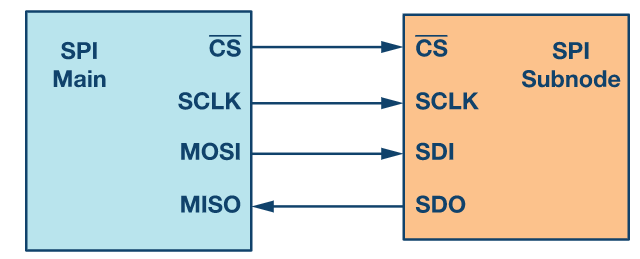
\includegraphics[width=0.5\textwidth]{figure/3_6.png}
    \caption{Connection between two devices using SPI}
    \label{fig:connection-spi}
\end{wrapfigure}
One of the most popular interfaces between micro-controllers and peripheral ICs, including sensors, ADCs, DACs, shift registers, SRAM, and others, is serial peripheral interface (SPI). The SPI interface is briefly explained. SPI is a main-subnode-based, synchronous, full-duplex interface. On the rising or falling clock edge, the data from the main node or the sub-node are synchronized. Data can be transmitted simultaneously by the main and sub-node. Both a 3-wire and a 4-wire SPI interface are available. When using more than sub-node, the forth pin is used since it is responsible for chip select as shown in figure \ref{fig:connection-spi}.\newline
The main must activate the CS signal, send the clock signal, and choose the sub-node before SPI communication can start. To pick the sub-node, the main must provide a logic 0 on the chip select signal, which is often an active low signal. Full-duplex SPI allows for simultaneous data transmission between the main and sub-node via the MOSI and MISO lines, respectively. Data is concurrently sent (shifted out serially onto the MOSI/SDO bus during SPI communication) and received (sampled or read in from the bus, MISO/SDI) during SPI communication. \newline
The shifting and sampling of the data are synchronized by the edge of the serial clock. The SPI interface gives the user the freedom to choose whether to sample and/or shift the data on the rising or falling edge of the clock. To find out how many data bits are sent over the SPI interface, please consult the device data sheet.

\subsubsection{SPI Pins}
SPI uses three pins for communication:
 MOSI, MISO and SCLK. MOSI is short for 
Master-Out-Slave-In and MISO stands for 
Master-In-Slave-Out. This shows that SPI
 uses master-slave scheme and operates 
at full duplex (simultaneous two-way communication). \newline
The SPI parameters, such as data rate, bit order, and mode, are set by the master device. The data rate is the SPI transmission speed, which is determined by the microcontroller's clock speed. The bit order specifies whether the first bit out is the rightmost (LSB) or leftmost (MSB). The next part delves deeper into the topic of mode. There can only be one master device, and the number of slaves is proportional to the number of Slave Select (SS) pins on the master device. When a master wishes to converse with a slave, the SS line to that slave is set to low, while the rest of the lines are set to high. After then, the data is read on the MOSI line, and the slave responds on the MISO line. Slaves have no direct communication with their fellow slaves. Pull-up resistors on SS pins are a solid design technique for efficiently isolating slave devices from one another’s is a de facto standard, albeit a sloppy one. As a result, device makers may implement the protocol in a variety of ways. It's a good idea to read the gadget datasheet beforehand. \newline

\subsubsection{SPI Interface}
A basic SPI connection uses the serial clock (SCK), Master Out Slave In (MOSI), Master in Slave Out (MISO), and Slave Select (SS) lines to link a master to slaves, as shown in figure \ref{fig:spi-integration}. Slaves can share the SCK, MOSI, and MISO signals, but each slave has its own SS line.
\begin{figure}[h]
   \centering
    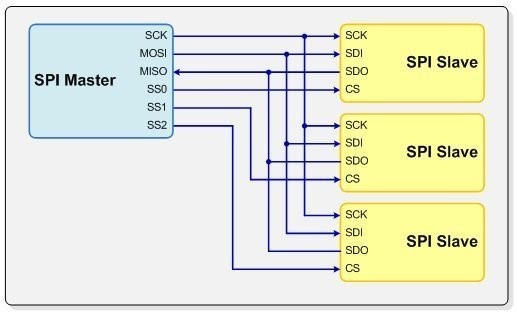
\includegraphics[width=.45\textwidth]{figure/3_7.jpg}
    \caption{SPI bus configuration with multiple slaves}
    \label{fig:spi-integration}
\end{figure}

\subsubsection{SPI Mode: Polarity and Clock Phase}
The SPI interface has no data exchange protocol, which reduces overhead and allows for high-speed data streaming. As shown in figure \ref{fig:spi-timing}, clock polarity (CPOL) and clock phase (CPHA) can be set to ‘0’ or ‘1’ to create four distinct modes for communication between master and slave.
\begin{figure}[h]
   \centering
    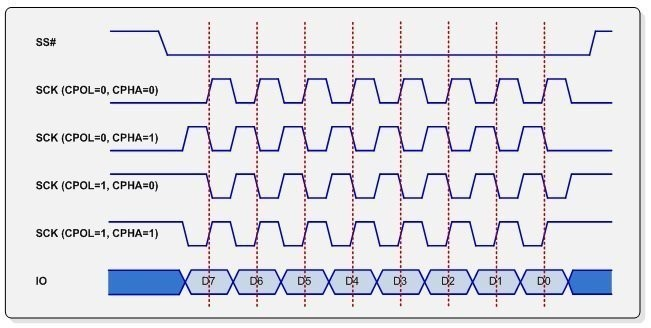
\includegraphics[width=\textwidth]{figure/3_8.jpg}
    \caption{SPI bus timing}
    \label{fig:spi-timing}
\end{figure}

As shown in figure \ref{fig:spi-modes}, Data is sampled at the leading rising edge of the clock if CPOL and CPHA are both ‘0’ (designated as Mode 0). SPI bus slave communication in mode 0 is by far the most prevalent. Data is sampled at the leading falling edge of the clock if CPOL is ‘1’ and CPHA is ‘0’ (Mode 2). Similarly, data sampled on the trailing falling edge with CPOL = ‘0’ and CPHA = ‘1’ (Mode 1), and data sampled on the trailing rising edge with CPOL = ‘1’ and CPHA = ‘1’ (Mode 3).

\begin{figure}[h]
   \centering
    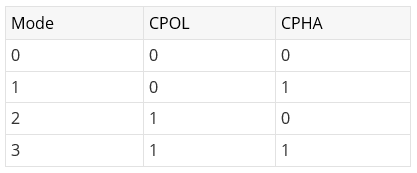
\includegraphics[width=\textwidth]{figure/3_9.PNG}
    \caption{SPI modes}
    \label{fig:spi-modes}
\end{figure}


\subsubsection{2. Why SPI is being used}
\begin{enumerate}
    \item Full duplex communication is supported.
    \item Because SPI uses a push-pull architecture, it can accommodate faster data speeds and longer distances.
    \item In comparison to I2C interface, it uses less power.
    \item Data can be transferred at high speed in tens of MHz.
\end{enumerate}

\subsubsection{3. Interfacing with SPI}
Although the ease of this protocol, it has a small role in the project since the used sensors and modules communicate with UART and I2C, so SPI driver is interacted with CAN module and raspberry pi to send and receive some data which will may need to display for the user.

\subsection{CAN}
Modern cars may feature up to 100 sensors and ECUs that must communicate and interact with one another in order to transfer data and monitor the vehicle's state. Microcontrollers and ECUs are increasing in number as more features are introduced to cars, such as smart car systems, autonomous driving systems, and V2X systems. Sensor devices provide information such as speed, position, and heat. As the information is vital to minimize accidents and traffic concerns, the Controller Area Network (CAN)communication protocol has been determined to be dependable to handle the communication with the lowest potential error. The Controller Area Network (CAN) standard is used to allow microcontrollers and devices in a vehicle to interact without the usage of a host computer. In many applications where several remote MCUs and sensors must interact with one another, such as industrial automation or robotics, the CAN bus provides a good communication protocol.

\subsubsection{1. Background of CAN}
The CAN bus was developed by BOSCH (1) as a multi-master, message broadcast system that specifies a maximum signaling rate of 1 megabit per second (bps). Unlike a traditional network such as USB or Ethernet, CAN does not send large blocks of data point-to-point from node A to node B under the supervision of a central bus master. In a CAN network, many short messages like temperature or RPM are broadcast to the entire network, which provides for data consistency in every node of the system. Once CAN basics such as message format, message identifiers, and bit-wise arbitration -- a major benefit of the CAN signaling scheme are explained, a CAN bus implementation is examined, typical waveforms presented, and transceiver features examined.

\subsubsection{The CAN Standard}
CAN is an International Standardization Organization (ISO) defined serial communications bus originally developed for the automotive industry to replace the complex wiring harness with a two-wire bus. The specification calls for high immunity to electrical interference and the ability to self-diagnose and repair data errors. These features have led to CAN’s popularity in a variety of industries including building automation, medical, and manufacturing. The CAN communications protocol, ISO-11898: 2003, describes how information is passed between devices on a network and conforms to the Open Systems Interconnection (OSI) model that is defined in terms of layers. Actual communication between devices connected by the physical medium is defined by the physical layer of the model. The ISO 11898 architecture defines the lowest two layers of the seven-layer OSI/ISO model as the data-link layer and physical layer in figure \ref{fig:iso-standard}.

\begin{figure}[h]
   \centering
    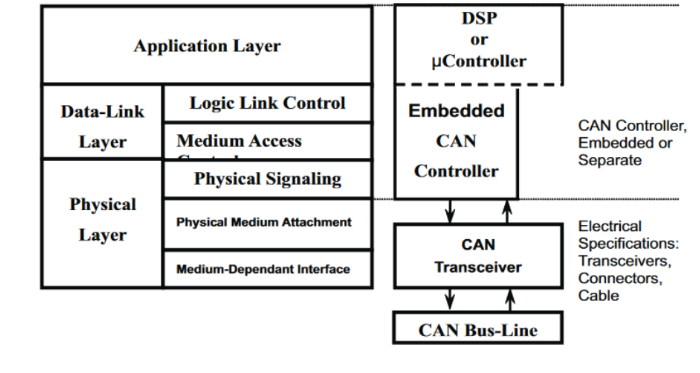
\includegraphics[width=\textwidth]{figure/3_10.png}
    \caption{The Layered ISO 11898 Standard Architecture. }
    \label{fig:iso-standard}
\end{figure}

\subsubsection{The Bit Fields of Standard CAN}
\begin{itemize}
    \item SOF - Start of Frame.
    \item 11-bit Identifier - establishes the priority of the message.
    \item  The lower the binary, the higher its priority.
    \item RTR - Remote Transmission Request is dominant
 when information is required from another node.
    \item IDE - Dominant single identifier extension bit means
 that a standard CAN identifier with no extension is being transmitted. 
 \item R0 – Reserved bit. 
 \item DLC – The 4-bit data length code. 
 \item Data – Up to 64 bits.
 \item CRC – The 16-bit cyclic redundancy check.
 \item ACK - Acknowledgment bit.
 \item EOF - End of Frame. 
 \item IFS – This 7-bit interframe space (IFS) contains the time 
required by the controller to move a correctly received frame 
to its proper position in a message buffer area.
\end{itemize}

\subsubsection{2. Why CAN is being used?}
A Controller Area Network (CAN) is ideally suitable for industrial communication protocols. Its cost, performance, and upgradeability provide high flexibility in system design. So, there is many advantages of CAN protocol.

\begin{enumerate}
    \item Low Cost
    \item Built-in Error Detection
    \item Robustness
    \item Speed
    \item Flexibility
\end{enumerate}

\subsubsection{3. Interfacing with CAN}
To interface between STM and can module, CAN bus must to implemented and integrated between them, and in order to make use of raspberry pi features, CAN module connects with raspberry using SPI protocol as shown in figure \ref{fig:interface-can}.
\begin{figure}[h]
   \centering
    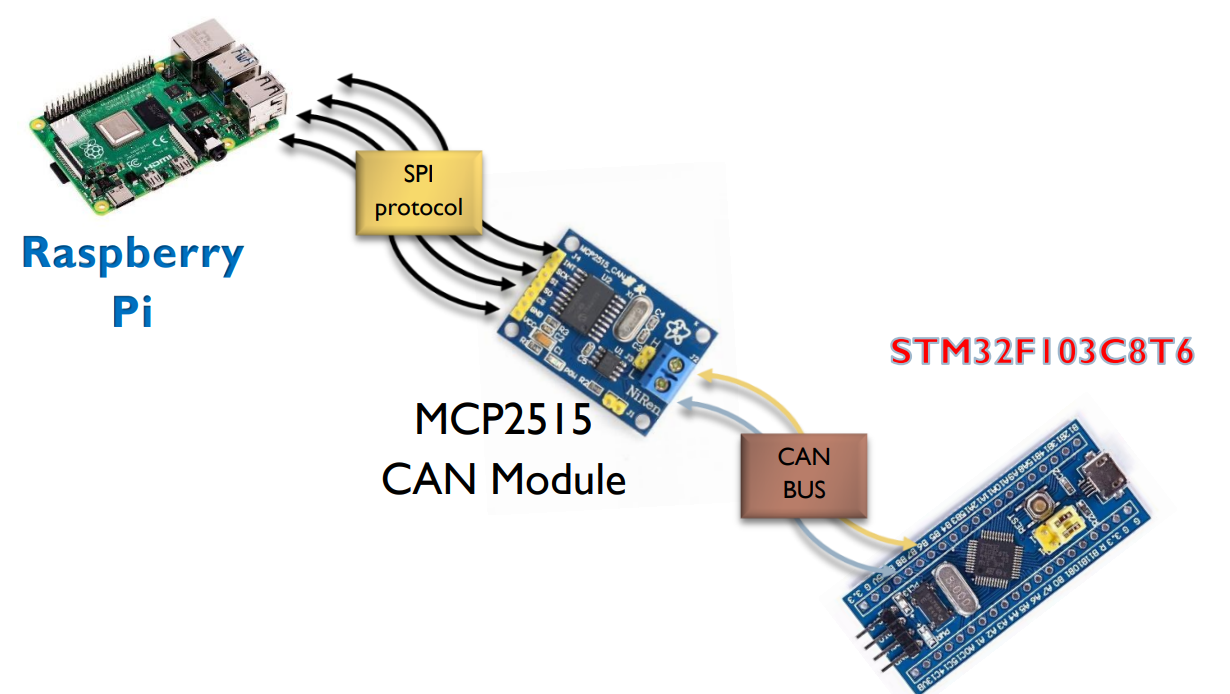
\includegraphics[width=\textwidth]{figure/3_11.png}
    \caption{Interfacing RP, STM32F103, and MCP2515 CAN Bus Module}
    \label{fig:interface-can}
\end{figure}

\section{Wireless Communication Protocols}
Wireless communication is needed to be able for V2V unit to communicate with the server and the mobile. In the following, Bluetooth and Wi-Fi will be discussed and how they are used in the project.

\subsection{Bluetooth}
Bluetooth is a short-range wireless technology; it can be used to exchange data between two devices in a short distance, so Bluetooth communication is a suitable choice to communicate between a mobile and the project. \newline
As discussed before, Bluetooth module was used to communicate with STM and in other side, it communicates with a mobile phone to give it all GPS data which includes longitude, latitude, and time. There are a lot of mobile software application that handle sharing GPS data from the mobile to any device has a Bluetooth module. \newline

Bluetooth is also used to communicate between the car prototype and the mobile to control the car motion remotely, it will be discussed in details in chapter 8.

\subsection{Wi-Fi}
Wi-Fi is a family of wireless network protocols, based on IEEE 802.11, Wi-Fi is suitable for wide range communication in a local area, so it is used for communicate between the vehicles and the server. \newline
To implement the connection, LAN network is integrated to connect a group of peripheral devices that share a common communications line or wireless link to a server within a distinct geographic area. \newline
Mentioned peripheral device in the project is Raspberry pi for each V2V unit since it has a Wi-Fi protocol. Details of this communication is discussed in chapter 6.

